\documentclass[10pt]{beamer}

% Packages
\usepackage[utf8]{inputenc}
\usepackage[T1]{fontenc}
\usepackage{amsmath, amssymb, amsthm}
\usepackage{graphicx}
\usepackage{booktabs}
\usepackage{hyperref}
\usepackage{tikz}
\usetikzlibrary{shapes,arrows,positioning}

% Theme settings
\usetheme{default}
\usecolortheme{default}
\usefonttheme{professionalfonts}

\definecolor{ImperialBlue}{RGB}{0, 62, 116}
\definecolor{DarkGray}{RGB}{51, 51, 51}
\definecolor{LightGray}{RGB}{245, 245, 245}
\definecolor{AccentOrange}{RGB}{214, 96, 77}
\definecolor{AccentGreen}{RGB}{46, 139, 87}

% Apply colors
\setbeamercolor{frametitle}{fg=ImperialBlue, bg=white}
\setbeamercolor{title}{fg=ImperialBlue}
\setbeamercolor{structure}{fg=ImperialBlue}
\setbeamercolor{normal text}{fg=DarkGray}
\setbeamercolor{block title}{fg=white, bg=ImperialBlue}
\setbeamercolor{block body}{fg=DarkGray, bg=LightGray}
\setbeamercolor{itemize item}{fg=ImperialBlue}
\setbeamercolor{enumerate item}{fg=ImperialBlue}

% Remove navigation symbols
\setbeamertemplate{navigation symbols}{}

% Customize frame title
\setbeamertemplate{frametitle}{
  \vspace{0.5em}
  \insertframetitle
  \vspace{0.3em}
}

% Customize itemize
\setbeamertemplate{itemize items}[circle]
\setlength{\leftmargini}{1.5em}

% Footer
\setbeamertemplate{footline}{
  \leavevmode%
  \hbox{%
  \begin{beamercolorbox}[wd=.333333\paperwidth,ht=2.25ex,dp=1ex,left]{author in head/foot}%
    \hspace{1em}\usebeamerfont{author in head/foot}\insertshortauthor
  \end{beamercolorbox}%
  \begin{beamercolorbox}[wd=.333333\paperwidth,ht=2.25ex,dp=1ex,center]{title in head/foot}%
    \usebeamerfont{title in head/foot}\insertshorttitle
  \end{beamercolorbox}%
  \begin{beamercolorbox}[wd=.333333\paperwidth,ht=2.25ex,dp=1ex,right]{date in head/foot}%
    \usebeamerfont{date in head/foot}\insertshortdate{}\hspace*{2em}
    \insertframenumber{} / \inserttotalframenumber\hspace*{2ex} 
  \end{beamercolorbox}}%
  \vskip0pt%
}

% Title page customization
\setbeamertemplate{title page}{
  \vbox{}
  \vfill
  \begingroup
    \centering
    {\usebeamercolor[fg]{title}\usebeamerfont{title}\inserttitle\par}
    \vskip0.5em
    {\usebeamercolor[fg]{subtitle}\usebeamerfont{subtitle}\insertsubtitle\par}
    \vskip2em
    {\usebeamercolor[fg]{author}\usebeamerfont{author}\insertauthor\par}
    \vskip0.5em
    {\usebeamercolor[fg]{institute}\usebeamerfont{institute}\insertinstitute\par}
    \vskip1em
    {\usebeamercolor[fg]{date}\usebeamerfont{date}\insertdate\par}
  \endgroup
  \vfill
}

% Commands for highlighting
\newcommand{\emphbox}[1]{\colorbox{LightGray}{\textcolor{DarkGray}{#1}}}
\newcommand{\highlight}[1]{\textcolor{AccentOrange}{\textbf{#1}}}
\newcommand{\good}[1]{\textcolor{AccentGreen}{#1}}
\newcommand{\bad}[1]{\textcolor{red}{#1}}

%----------------------------------------------------------------------------------------
\title{Foundations of Blockchain Technology}
\subtitle{ECOM215: Blockchain Economics and Digital Assets}
\author{Dr Daniele Bianchi}
\institute{Queen Mary, University of London}
\date{Semester B, 2025/2026}
%----------------------------------------------------------------------------------------

\begin{document}

\AtBeginSection[]{
  \begin{frame}[plain]
    \vfill
    \begin{center}
      {\Large\color{ImperialBlue}\insertsection}
    \end{center}
    \vfill
  \end{frame}
}

\begin{frame}[plain]
  \titlepage
\end{frame}

\begin{frame}{Today's Agenda}
  \tableofcontents
\end{frame}

%----------------------------------------------------------------------------------------
\section{Why Blockchain Matters}
%----------------------------------------------------------------------------------------

\begin{frame}{A Simple Problem: Sending Money Abroad}
  \begin{center}
    \Large You want to send £1,000 to a relative in another country.
  \end{center}
  
  \vspace{1.5em}
  \textbf{What happens with traditional banking:}
  \begin{enumerate}
    \item Your bank verifies your identity and balance
    \item Your bank contacts correspondent banks (often 2--3 intermediaries)
    \item Each intermediary verifies the transaction and extracts a fee
    \item Settlement takes 2--5 business days
    \item Total cost: 5--10\% of the transfer amount
  \end{enumerate}
  
  \vspace{1em}
  \textbf{The core problem:} Each institution maintains its own ledger. Reconciling across ledgers requires \highlight{trust}, \highlight{time}, and \highlight{money}.
\end{frame}

\begin{frame}{The Role of Intermediaries}
  Most economic transactions rely on \highlight{trusted third parties}:
  
  \vspace{0.5em}
  \begin{itemize}
    \item Banks verify balances and process payments
    \item Lawyers and notaries certify contracts
    \item Credit card networks guarantee merchant payments
    \item Governments maintain registries (land, identity, vehicles)
  \end{itemize}
  
  \vspace{1em}
  These intermediaries provide valuable services, but introduce:
  
  \vspace{0.5em}
  \begin{center}
  \begin{tabular}{ll}
    \toprule
    \textbf{Issue} & \textbf{Example} \\
    \midrule
    \bad{Costs} & Processing fees, compliance overhead \\
    \bad{Delays} & Settlement times, reconciliation \\
    \bad{Single points of failure} & Outages, fraud, insolvency \\
    \bad{Exclusion} & 1.4 billion adults lack bank access \\
    \bottomrule
  \end{tabular}
  \end{center}
\end{frame}

\begin{frame}{The Blockchain Proposition}
  \begin{block}{What if...}
    \begin{itemize}
      \item A single shared ledger recorded all transactions
      \item Anyone could verify the ledger's accuracy independently
      \item No single party could control or manipulate records
      \item Transactions settled in minutes, not days
      \item The system operated 24/7 without institutional downtime
    \end{itemize}
  \end{block}
  
  \vspace{1em}
  This is the core idea: replace \highlight{trust in institutions} with \highlight{trust in a transparent, decentralised system}.
  
  \vspace{1em}
  \textbf{The critical question for this course:}
  
  When does this proposition deliver real economic value---and when is it hype?
\end{frame}

\begin{frame}{Blockchain: From Experiment to Infrastructure}
  Blockchain is no longer ``emerging technology.'' Key milestones:
  
  \vspace{0.5em}
  \begin{center}
  \begin{tabular}{cl}
    \toprule
    \textbf{Year} & \textbf{Development} \\
    \midrule
    2009 & Bitcoin launches (peer-to-peer electronic cash) \\
    2015 & Ethereum introduces programmable smart contracts \\
    2017--20 & Enterprise pilots (supply chain, trade finance) \\
    2020--23 & DeFi growth, stablecoins reach \$100B+ \\
    2024 & \good{Bitcoin \& Ethereum spot ETFs approved (US)} \\
    2024 & \good{MiCA regulation enters force (EU)} \\
    \bottomrule
  \end{tabular}
  \end{center}
  
  \vspace{1em}
  Today: crypto market cap $>$\$2 trillion, institutional custody solutions, regulated investment products, comprehensive legal frameworks.
\end{frame}

%----------------------------------------------------------------------------------------
\section{What is Blockchain?}
%----------------------------------------------------------------------------------------

\begin{frame}{Blockchain: A Definition}
  \begin{block}{Definition}
    A \textbf{blockchain} is a distributed digital ledger that records transactions in linked groups (blocks), secured by cryptography, maintained by a network of computers without central control.
  \end{block}
  
  \vspace{1em}
  Four foundational components:
  
  \vspace{0.5em}
  \begin{enumerate}
    \item \textbf{Cryptography} --- secures data and verifies identity
    \item \textbf{Data structure} --- organises transactions into linked blocks
    \item \textbf{Distributed network} --- replicates ledger across many nodes
    \item \textbf{Economic incentives} --- motivates honest participation
  \end{enumerate}
  
  \vspace{1em}
  Think of it as a \highlight{cleverly designed bookkeeping system} where the bookkeepers don't need to trust each other.
\end{frame}

\begin{frame}{The Chain of Blocks}
  % [FIGURE NEEDED: Clean diagram showing blocks linked by hashes]
  % Suggested source: Create TikZ diagram or use Glassnode/educational materials
  
  \begin{center}
  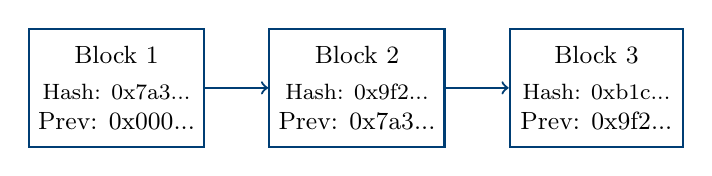
\begin{tikzpicture}[
    block/.style={rectangle, draw=ImperialBlue, thick, minimum width=2.2cm, minimum height=1.5cm, align=center, font=\small},
    arrow/.style={->, thick, ImperialBlue}
  ]
    \node[block] (b1) {Block 1\\[0.2em]\footnotesize Hash: 0x7a3...\\Prev: 0x000...};
    \node[block, right=0.8cm of b1] (b2) {Block 2\\[0.2em]\footnotesize Hash: 0x9f2...\\Prev: 0x7a3...};
    \node[block, right=0.8cm of b2] (b3) {Block 3\\[0.2em]\footnotesize Hash: 0xb1c...\\Prev: 0x9f2...};
    
    \draw[arrow] (b1) -- (b2);
    \draw[arrow] (b2) -- (b3);
  \end{tikzpicture}
  \end{center}
  
  \vspace{1em}
  \textbf{Key insight:} Each block contains the cryptographic ``signature'' (hash) of the previous block.
  
  \begin{itemize}
    \item If someone modifies Block 1, its hash changes
    \item Block 2's ``previous hash'' no longer matches
    \item The tampering is immediately detectable
  \end{itemize}

  \vspace{1em}
  This creates \highlight{immutability}: changing history requires rewriting the entire chain.
\end{frame}

\begin{frame}{Key Terminology}
  \begin{block}{Distributed Ledger}
    An append-only database replicated across many network nodes. New records can be added; existing records cannot be modified or deleted.
  \end{block}
  
  \vspace{0.5em}
  \begin{block}{Block}
    A batch of transactions recorded together. Block size and timing vary by blockchain (Ethereum: variable size every 12 seconds).
  \end{block}
  
  \vspace{0.5em}
  \begin{block}{Node}
    A computer participating in the network. \textbf{Full nodes} store the complete ledger and independently validate all transactions. \textbf{Light nodes} store only block headers and query full transaction data as needed.
  \end{block}
  
  \vspace{0.5em}
  \begin{block}{Consensus Protocol}
    The rules by which nodes agree on ledger updates. Examples: Proof-of-Work, Proof-of-Stake (covered in Topic 2).
  \end{block}
\end{frame}

\begin{frame}{How a Transaction Works}
  \begin{center}
  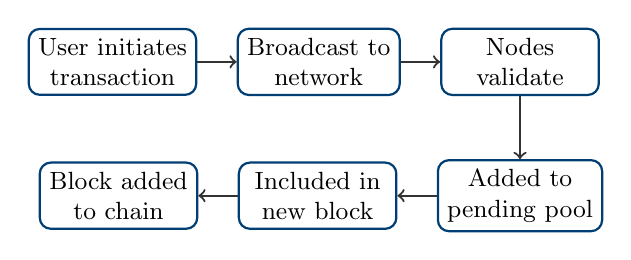
\begin{tikzpicture}[
    node distance=0.7cm,
    box/.style={draw=ImperialBlue, thick, rectangle, rounded corners, minimum width=2cm, minimum height=0.8cm, align=center, font=\small},
    arrow/.style={->, thick, DarkGray}
  ]
    \node[box] (1) {User initiates\\transaction};
    \node[box, right=0.5cm of 1] (2) {Broadcast to\\network};
    \node[box, right=0.5cm of 2] (3) {Nodes\\validate};
    \node[box, below=0.8cm of 3] (4) {Added to\\pending pool};
    \node[box, left=0.5cm of 4] (5) {Included in\\new block};
    \node[box, left=0.5cm of 5] (6) {Block added\\to chain};
    
    \draw[arrow] (1) -- (2);
    \draw[arrow] (2) -- (3);
    \draw[arrow] (3) -- (4);
    \draw[arrow] (4) -- (5);
    \draw[arrow] (5) -- (6);
  \end{tikzpicture}
  \end{center}
  
  \vspace{1em}
  \textbf{Critical points:}
  \begin{itemize}
    \item Validation happens \textit{before} recording (integrity)
    \item Once recorded, transactions cannot be reversed (irreversibility)
    \item All nodes receive the same updated ledger (transparency)
    \item No central authority approves transactions (decentralisation)
  \end{itemize}
\end{frame}

%----------------------------------------------------------------------------------------
\section{Cryptographic Foundations}
%----------------------------------------------------------------------------------------

\begin{frame}{Why Cryptography?}
  Blockchain relies on cryptographic tools to solve specific problems:
  
  \vspace{1em}
  \textbf{1. Integrity} --- Has the data been tampered with?
  \begin{itemize}
    \item Hash functions produce a unique ``fingerprint'' of data
    \item Any modification, however small, changes the fingerprint completely
  \end{itemize}
  
  \vspace{0.5em}
  \textbf{2. Authentication} --- Who authorised this transaction?
  \begin{itemize}
    \item Digital signatures can only be created with the sender's private key
    \item Anyone can verify the signature using the sender's public key
  \end{itemize}
  
  \vspace{0.5em}
  \textbf{3. Transparency, not confidentiality}
  \begin{itemize}
    \item Public blockchains do \textit{not} encrypt transaction data
    \item Anyone can see amounts and addresses (pseudonymous, not anonymous)
  \end{itemize}
\end{frame}

\begin{frame}{Hash Functions}
  \begin{block}{Definition}
    A \textbf{hash function} takes input of any size and produces a fixed-length output (the ``hash'' or ``digest''). Small input changes produce completely different outputs.
  \end{block}
  
  \vspace{0.5em}
  \textbf{Example} (SHA-256, used by Bitcoin):
  
  \vspace{0.3em}
  \texttt{\small "Hello" → 185f8db32271fe25f561a6fc938b2e26...}
  
  \texttt{\small "Hello." → f52fbd32b2b3b86ff88ef6c490628285...}
  
  \vspace{1em}
  \textbf{Key properties:}
  \begin{itemize}
    \item \textbf{Deterministic}: Same input always gives same output
    \item \textbf{One-way}: Cannot recover input from output
    \item \textbf{Collision-resistant}: Practically impossible to find two inputs with the same hash
    \item \textbf{Avalanche effect}: Tiny input change $\rightarrow$ completely different hash
  \end{itemize}
\end{frame}

\begin{frame}{Hash Functions in Blockchain}
  Hashes serve multiple purposes:

  \vspace{0.5em}
  \textbf{1. Linking blocks}
  \begin{itemize}
    \item Each block header is hashed to produce a \textit{block hash}
    \item This block hash is included in the next block's header
  \end{itemize}

  \vspace{0.5em}
  \textbf{2. Identifying transactions}
  \begin{itemize}
    \item Each transaction is hashed to produce a \textit{transaction ID}
    \item All transaction hashes in a block are combined into a \textit{Merkle tree}
    \item The Merkle root is included in the block header---so the block hash commits to every transaction
  \end{itemize}

  \vspace{0.5em}
  \textbf{3. Proof-of-Work} (Topic 2)
  \begin{itemize}
    \item Miners must find inputs that produce hashes meeting specific criteria
  \end{itemize}
\end{frame}

\begin{frame}{Public-Key Cryptography}
  \begin{block}{The Problem}
    How can two parties communicate securely without first meeting to share a secret key?
  \end{block}
  
  \vspace{0.5em}
  \textbf{Solution: Asymmetric encryption}
  
  Each user has a \highlight{key pair}:
  \begin{itemize}
    \item \textbf{Public key}: Shared openly (like an email address)
    \item \textbf{Private key}: Kept secret (like a password)
  \end{itemize}
  
  \vspace{1em}
  \textbf{Two uses:}
    \vspace{-1.5em}
  \begin{center}
  \resizebox{1\textwidth}{!}{\begin{tabular}{lll}
    \toprule
    \textbf{Operation} & \textbf{Encrypt with} & \textbf{Decrypt with} \\
    \midrule
    Sending private message & Recipient's public key & Recipient's private key \\
    Signing a transaction & Sender's private key & Sender's public key \\
    \bottomrule
  \end{tabular}}
  \end{center}
\end{frame}

\begin{frame}{Digital Signatures in Blockchain}
  When you send cryptocurrency:
  \vspace{0.5em}
  \begin{enumerate}
    \item You create a transaction message (``send 1 BTC to address X'')
    \item You sign it with your \highlight{private key}
    \item The network verifies the signature using your \highlight{public key}
  \end{enumerate}
  
  \vspace{1em}
  \textbf{What this guarantees:}
  \begin{itemize}
    \item \good{\bf Authentication}: Only the private key holder could have signed
    \item \good{\bf Integrity}: Any modification invalidates the signature
    \item \good{\bf Non-repudiation}: Signer cannot deny the transaction
  \end{itemize}
  
  \vspace{1em}
  \textbf{Critical implication:}
  
  \bad{If you lose your private key, you lose access to your assets.}
  
  \bad{If someone steals your private key, they control your assets.}
  
  There is no ``forgot password'' reset. This is a feature, not a bug.
\end{frame}

%----------------------------------------------------------------------------------------
\section{Core Properties of Blockchain}
%----------------------------------------------------------------------------------------

\begin{frame}{The Five Properties}
  Different blockchains achieve these properties to different degrees:
  
  \vspace{1em}
  \begin{enumerate}
    \item \textbf{Immutability}: Recorded transactions cannot be altered
    
    \item \textbf{Irreversibility}: Confirmed transactions cannot be undone
    
    \item \textbf{Integrity}: Only valid transactions are recorded
    
    \item \textbf{Transparency}: Transaction history is publicly auditable
    
    \item \textbf{Decentralisation}: No single point of control or failure
  \end{enumerate}
  
  \vspace{1em}
  \begin{block}{The Blockchain Trilemma (Topic 2)}
    It is difficult to simultaneously maximise \highlight{decentralisation}, \highlight{security}, and \highlight{scalability}. Design choices involve trade-offs.
  \end{block}
\end{frame}

\begin{frame}{Immutability and Irreversibility}
  \textbf{Immutability}: The ledger's history cannot be rewritten.
  
  \begin{itemize}
    \item Guaranteed by hash-linking of blocks
    \item Changing old data requires re-mining all subsequent blocks
    \item Economically prohibitive on large networks
  \end{itemize}
  
  \vspace{1em}
  \textbf{Irreversibility}: Transactions cannot be ``undone.''
  
  \begin{itemize}
    \item Critical for preventing double-spending
    \item If you send funds to the wrong address, there is no reversal mechanism
    \item Contrast with credit cards (chargebacks) or bank transfers (recalls)
  \end{itemize}
  
  \vspace{1em}
  \textbf{Implication}: Blockchain is well-suited for situations where finality is valuable (settlement, proof of existence) but creates challenges for error correction.
\end{frame}

\begin{frame}{Transparency and Decentralisation}
  \textbf{Transparency}: All transactions are visible to all participants.
  
  \begin{itemize}
    \item Anyone can audit the complete transaction history
    \item Builds trust without requiring trust in any single party
    \item \bad{Privacy trade-off}: Pseudonymous, not anonymous
  \end{itemize}
  
  \vspace{1em}
  \textbf{Decentralisation}: No central authority controls the network.
  
  \begin{itemize}
    \item Thousands of independent nodes maintain the ledger
    \item No single point of failure or censorship
    \item Decisions made through protocol rules and consensus
  \end{itemize}
  
  \vspace{1em}
  \textbf{Key insight}: These properties are \textit{emergent}---they arise from the system design, not from any guarantee by a trusted party. The system is only as robust as its weakest design assumption.
\end{frame}


\begin{frame}{Public vs Private vs Consortium}

\highlight{We can distinguish different types of blockchains.}

  \begin{center}
  \resizebox{1\textwidth}{!}{\begin{tabular}{lccc}
    \toprule
    & \textbf{Public} & \textbf{Consortium} & \textbf{Private} \\
    \midrule
    Access & Open to all & Invited orgs & Single org \\
    Consensus & Permissionless & Pre-selected nodes & Centralised \\
    Speed & \bad{Slower} & Medium & \good{Fastest} \\
    Decentralisation & \good{High} & Medium & \bad{Low} \\
    Examples & Bitcoin, Ethereum & R3 Corda, Hyperledger & Internal DBs \\
    \bottomrule
  \end{tabular}}
  \end{center}
  
  \vspace{1em}
  \highlight{The trade-off}:
  \begin{itemize}
    \item Public chains maximise trust minimisation but sacrifice throughput
    \item Private chains maximise efficiency but require trusting the operator
    \item Consortium chains attempt a middle ground
  \end{itemize}
\end{frame}

\begin{frame}{Public Blockchains}
  \textbf{Definition}: Open networks where anyone can participate, validate, and audit.
  
  \vspace{0.5em}
  \textbf{Examples}: Bitcoin, Ethereum, Solana
  
  \vspace{1em}
  \good{Advantages:}
  \begin{itemize}
    \item Maximum decentralisation and censorship resistance
    \item Trustless: security from protocol, not institutions
    \item Permissionless innovation: anyone can build on top
  \end{itemize}
  
  \vspace{0.5em}
  \bad{Disadvantages:}
  \begin{itemize}
    \item Scalability constraints (throughput, latency)
    \item Energy consumption (Proof-of-Work) or capital requirements (Proof-of-Stake)
    \item Governance challenges for protocol upgrades
  \end{itemize}
  
  \vspace{0.5em}
  \textbf{Note}: Layer 2 solutions (Topic 2) address scalability by processing transactions off the main chain while inheriting its security.
\end{frame}

\begin{frame}{Private and Consortium Blockchains}
  \textbf{Private blockchain}: Controlled by a single organisation.
  
  \begin{itemize}
    \item Fast and efficient (fewer nodes, simpler consensus)
    \item Full control over access and governance
    \item \bad{But}: Requires trusting the operator---arguably ``just a database''
  \end{itemize}
  
  \vspace{1em}
  \textbf{Consortium blockchain}: Controlled by a group of organisations.
  
  \begin{itemize}
    \item Shared infrastructure without full public exposure
    \item Useful when multiple parties need a common record but don't fully trust each other
    \item Examples: Trade finance (we.trade), securities settlement (DTCC)
  \end{itemize}
  
  \vspace{1em}
  \textbf{When do these make sense?}
  
  When you need auditability and coordination across organisations, but public transparency is undesirable or regulatory constraints apply.
\end{frame}

%----------------------------------------------------------------------------------------
\section{Use Cases Beyond Cryptocurrency}
%----------------------------------------------------------------------------------------

\begin{frame}{Where Blockchain Adds Value}
  Blockchain is most useful when:
  
  \vspace{0.5em}
  \begin{itemize}
    \item Multiple parties need a \highlight{shared record}
    \item Those parties don't fully \highlight{trust each other}
    \item A trusted intermediary is \highlight{costly, slow, or unavailable}
    \item \highlight{Auditability} and \highlight{tamper-evidence} are valuable
  \end{itemize}
  
  \vspace{1em}
  Blockchain is \textit{not} useful when:
  
  \vspace{0.5em}
  \begin{itemize}
    \item A single organisation controls all data
    \item Participants already trust each other
    \item Speed is critical and finality can wait
    \item Data needs to be frequently modified or deleted
  \end{itemize}
  
  \vspace{1em}
  \textbf{Rule of thumb}: If a traditional database solves the problem, use a database. Blockchain adds value through trust minimisation, not raw performance.
\end{frame}

\begin{frame}{Supply Chain Management}
  \textbf{Problem}: Tracking goods across multiple parties (manufacturers, shippers, customs, retailers) with no single trusted record-keeper.
  
  \vspace{1em}
  \textbf{Blockchain solution}:
  \begin{itemize}
    \item Shared ledger records provenance and chain of custody
    \item Each handoff is cryptographically signed
    \item Smart contracts can automate payments upon delivery confirmation
  \end{itemize}
  
  \vspace{1em}
  \textbf{Examples}:
  \begin{itemize}
    \item IBM Food Trust: Walmart traces produce from farm to shelf
    \item TradeLens (Maersk + IBM): Container shipping documentation
    \item De Beers (Tracr): Diamond provenance verification
  \end{itemize}
  
  \vspace{1em}
  \textbf{Limitation}: Blockchain guarantees data integrity \textit{on-chain}, but cannot verify that off-chain inputs are accurate (``garbage in, garbage out'').
\end{frame}

\begin{frame}{Financial Services}
  \textbf{Settlement and clearing}:
  \begin{itemize}
    \item Traditional securities settlement: T+2 (trade date + 2 days)
    \item Blockchain-based settlement: potentially near-instant
    \item Reduces counterparty risk and capital requirements
  \end{itemize}
  
  \vspace{0.5em}
  \textbf{Trade finance}:
  \begin{itemize}
    \item Letters of credit, bills of lading still largely paper-based
    \item Consortium blockchains digitise and automate documentation
  \end{itemize}
  
  \vspace{0.5em}
  \textbf{Cross-border payments}:
  \begin{itemize}
    \item Correspondent banking is slow and expensive
    \item Stablecoins and CBDCs offer alternatives (Topics 4--5)
  \end{itemize}
  
  \vspace{1em}
  \textbf{We will cover these in depth}: DeFi (Topic 4), Stablecoins and CBDCs (Topic 5), Tokenisation of real-world assets (Topic 9).
\end{frame}

\begin{frame}{Identity and Government Services}
  \textbf{Digital identity}:
  \begin{itemize}
    \item Self-sovereign identity: users control their own credentials
    \item Verifiable credentials without revealing underlying data
    \item Estonia's e-Residency programme uses blockchain-backed identity
  \end{itemize}
  
  \vspace{0.5em}
  \textbf{Land registries}:
  \begin{itemize}
    \item Immutable record of property ownership
    \item Reduces fraud and disputes in developing economies
    \item Georgia, Sweden, Dubai have piloted blockchain registries
  \end{itemize}
  
  \vspace{0.5em}
  \textbf{Voting}:
  \begin{itemize}
    \item Transparent, auditable vote records
    \item \bad{Significant security and privacy challenges remain}
    \item Corporate shareholder voting more tractable than political elections
  \end{itemize}
\end{frame}

%----------------------------------------------------------------------------------------
\section{Summary and Next Steps}
%----------------------------------------------------------------------------------------

\begin{frame}{Key Takeaways}
  \begin{enumerate}
    \item \textbf{Blockchain enables coordination without trusted intermediaries}
    \begin{itemize}
      \item Useful when multiple parties need shared, tamper-evident records
    \end{itemize}
    
    \vspace{0.3em}
    \item \textbf{Core mechanism: cryptographically linked blocks}
    \begin{itemize}
      \item Hash functions ensure integrity; digital signatures ensure authenticity
    \end{itemize}
    
    \vspace{0.3em}
    \item \textbf{Key properties: immutability, transparency, decentralisation}
    \begin{itemize}
      \item But there are trade-offs (the blockchain trilemma)
    \end{itemize}
    
    \vspace{0.3em}
    \item \textbf{Different blockchains serve different purposes}
    \begin{itemize}
      \item Public (trust minimisation) vs private/consortium (efficiency)
    \end{itemize}
    
    \vspace{0.3em}
    \item \textbf{Use cases extend beyond cryptocurrency}
    \begin{itemize}
      \item Supply chain, financial settlement, identity, governance
    \end{itemize}
  \end{enumerate}
\end{frame}

\begin{frame}{What's Next}
  \textbf{Topic 2: Blockchain Economics}
  \begin{itemize}
    \item Consensus mechanisms: Proof-of-Work vs Proof-of-Stake
    \item The blockchain trilemma: decentralisation, security, scalability
    \item Economic incentives: mining, staking, fee markets
    \item Energy consumption and environmental concerns
  \end{itemize}
  
  \vspace{1em}
  \textbf{Preparation}:
  \begin{itemize}
    \item Review: What problem does consensus solve in a decentralised network?
    \item Think about: What incentives would motivate strangers to honestly maintain a shared ledger?
  \end{itemize}
\end{frame}

\begin{frame}[plain]
  \vfill
  \begin{center}
    {\Large Questions?}
  \end{center}
  \vfill
\end{frame}

\end{document}